\chapter{Materials and Methods}
\label{chap:materials-and-methods}

This chapter deals with background information relevant for your thesis, including physiological background, existing research on the topic, and mathematical and other preliminaries required to understand the novel concepts presented in the following chapter.

\section{\LaTeX's Features}

This section gives some useful hints to write a thesis with \LaTeX. 
It is important to know that \LaTeX\ is not a WYSIWYG (what you see is what you get) program like other text editors, such as Microsoft Word.
Instead, it much more resembles a programming language, in which you construct your text by proper usage of syntax.
The ``source code'' is your \LaTeX\ file (\texttt{.tex}). 

As in other programming languages, it is possible to insert comments in \LaTeX\ that are not visible in the final text. 
Line wraps are not of importance while writing the text, since they are created during compilation.
Therefore, formatting with \LaTeX\ is not a big deal and should not take a lot of time, if all the logical relations are correct.

One of the big advantages of \LaTeX\ is its strong support for typesetting mathematical formulas. 
Using the logical referencing of your formulas, those references are always correct, even if you change the position of the formulas. 
Furthermore the print quality you achieve with \LaTeX\ formulas is hardly matched by any other program, let alone free of charge!
Citing other works and providing a nicely compiled list of references is very easy in \LaTeX, as well.

The following text is not very meaningful on its own, but if you read the source code at the same time, it is easy to understand how different elements are constructed. 
You should try to compile the file yourself and compare the results. 
If there are any differences, check if your \LaTeX\ configuration is correct.

\section{Getting started with Latex}
\label{sec:getting-started-with}

To get started with Latex, you need...
\begin{enumerate}
\item a tool that generates a PDF file out of a bunch of *.tex and *.bib files.
In Windows, this is typically \swname{MikTex} (\url{http://miktex.org/download}).
\item a text editor. This can be as simple as \swname{Notepad++} (\url{https://notepad-plus-plus.org/}), but many would recommend an IDE that provides further convenience features. \swname{TexMaker} (\url{http://www.heise.de/download/texmaker.html}) and \swname{TexStudio} (\url{http://www.texstudio.org/}) are two well-known examples.
\end{enumerate}
If you have these two installed on your PC, you're ready to go!
There is a wealth of references and tutorials on the internet that deal with Latex.
What follows is a small list compiled based on my personal preferences.
\begin{itemize}
\item ShareLatex currently provides - to my taste - the best introduction and reference on a number of Latex-related topics: \url{https://www.sharelatex.com/learn}.
\item Latex-Wikibooks often prove useful if you're really looking for a reference of the available symbols, e.g. \url{https://en.wikibooks.org/wiki/LaTeX/Mathematics} or \url{https://en.wikibooks.org/wiki/LaTeX/Tables}.
\item There is a neat little online tool available, which provides users with hints on available Latex commands based on the user's drawing of the desired symbol: \url{http://detexify.kirelabs.org/classify.html}.
\item Malte Schmitz from the Universität Lübeck also provides good introductory material in German: \url{http://www.mlte.de/layout}.
\end{itemize}


\section{Figures in Latex}
\Cref{fig:sfap-schematic} shows a schematic of the geometry of of \gls{sfap} detection.
Note the extensive figure caption: many readers will first skim through your thesis and look at the figures, which should hence be as self-explanatory as possible.
\begin{figure}
  \centering
  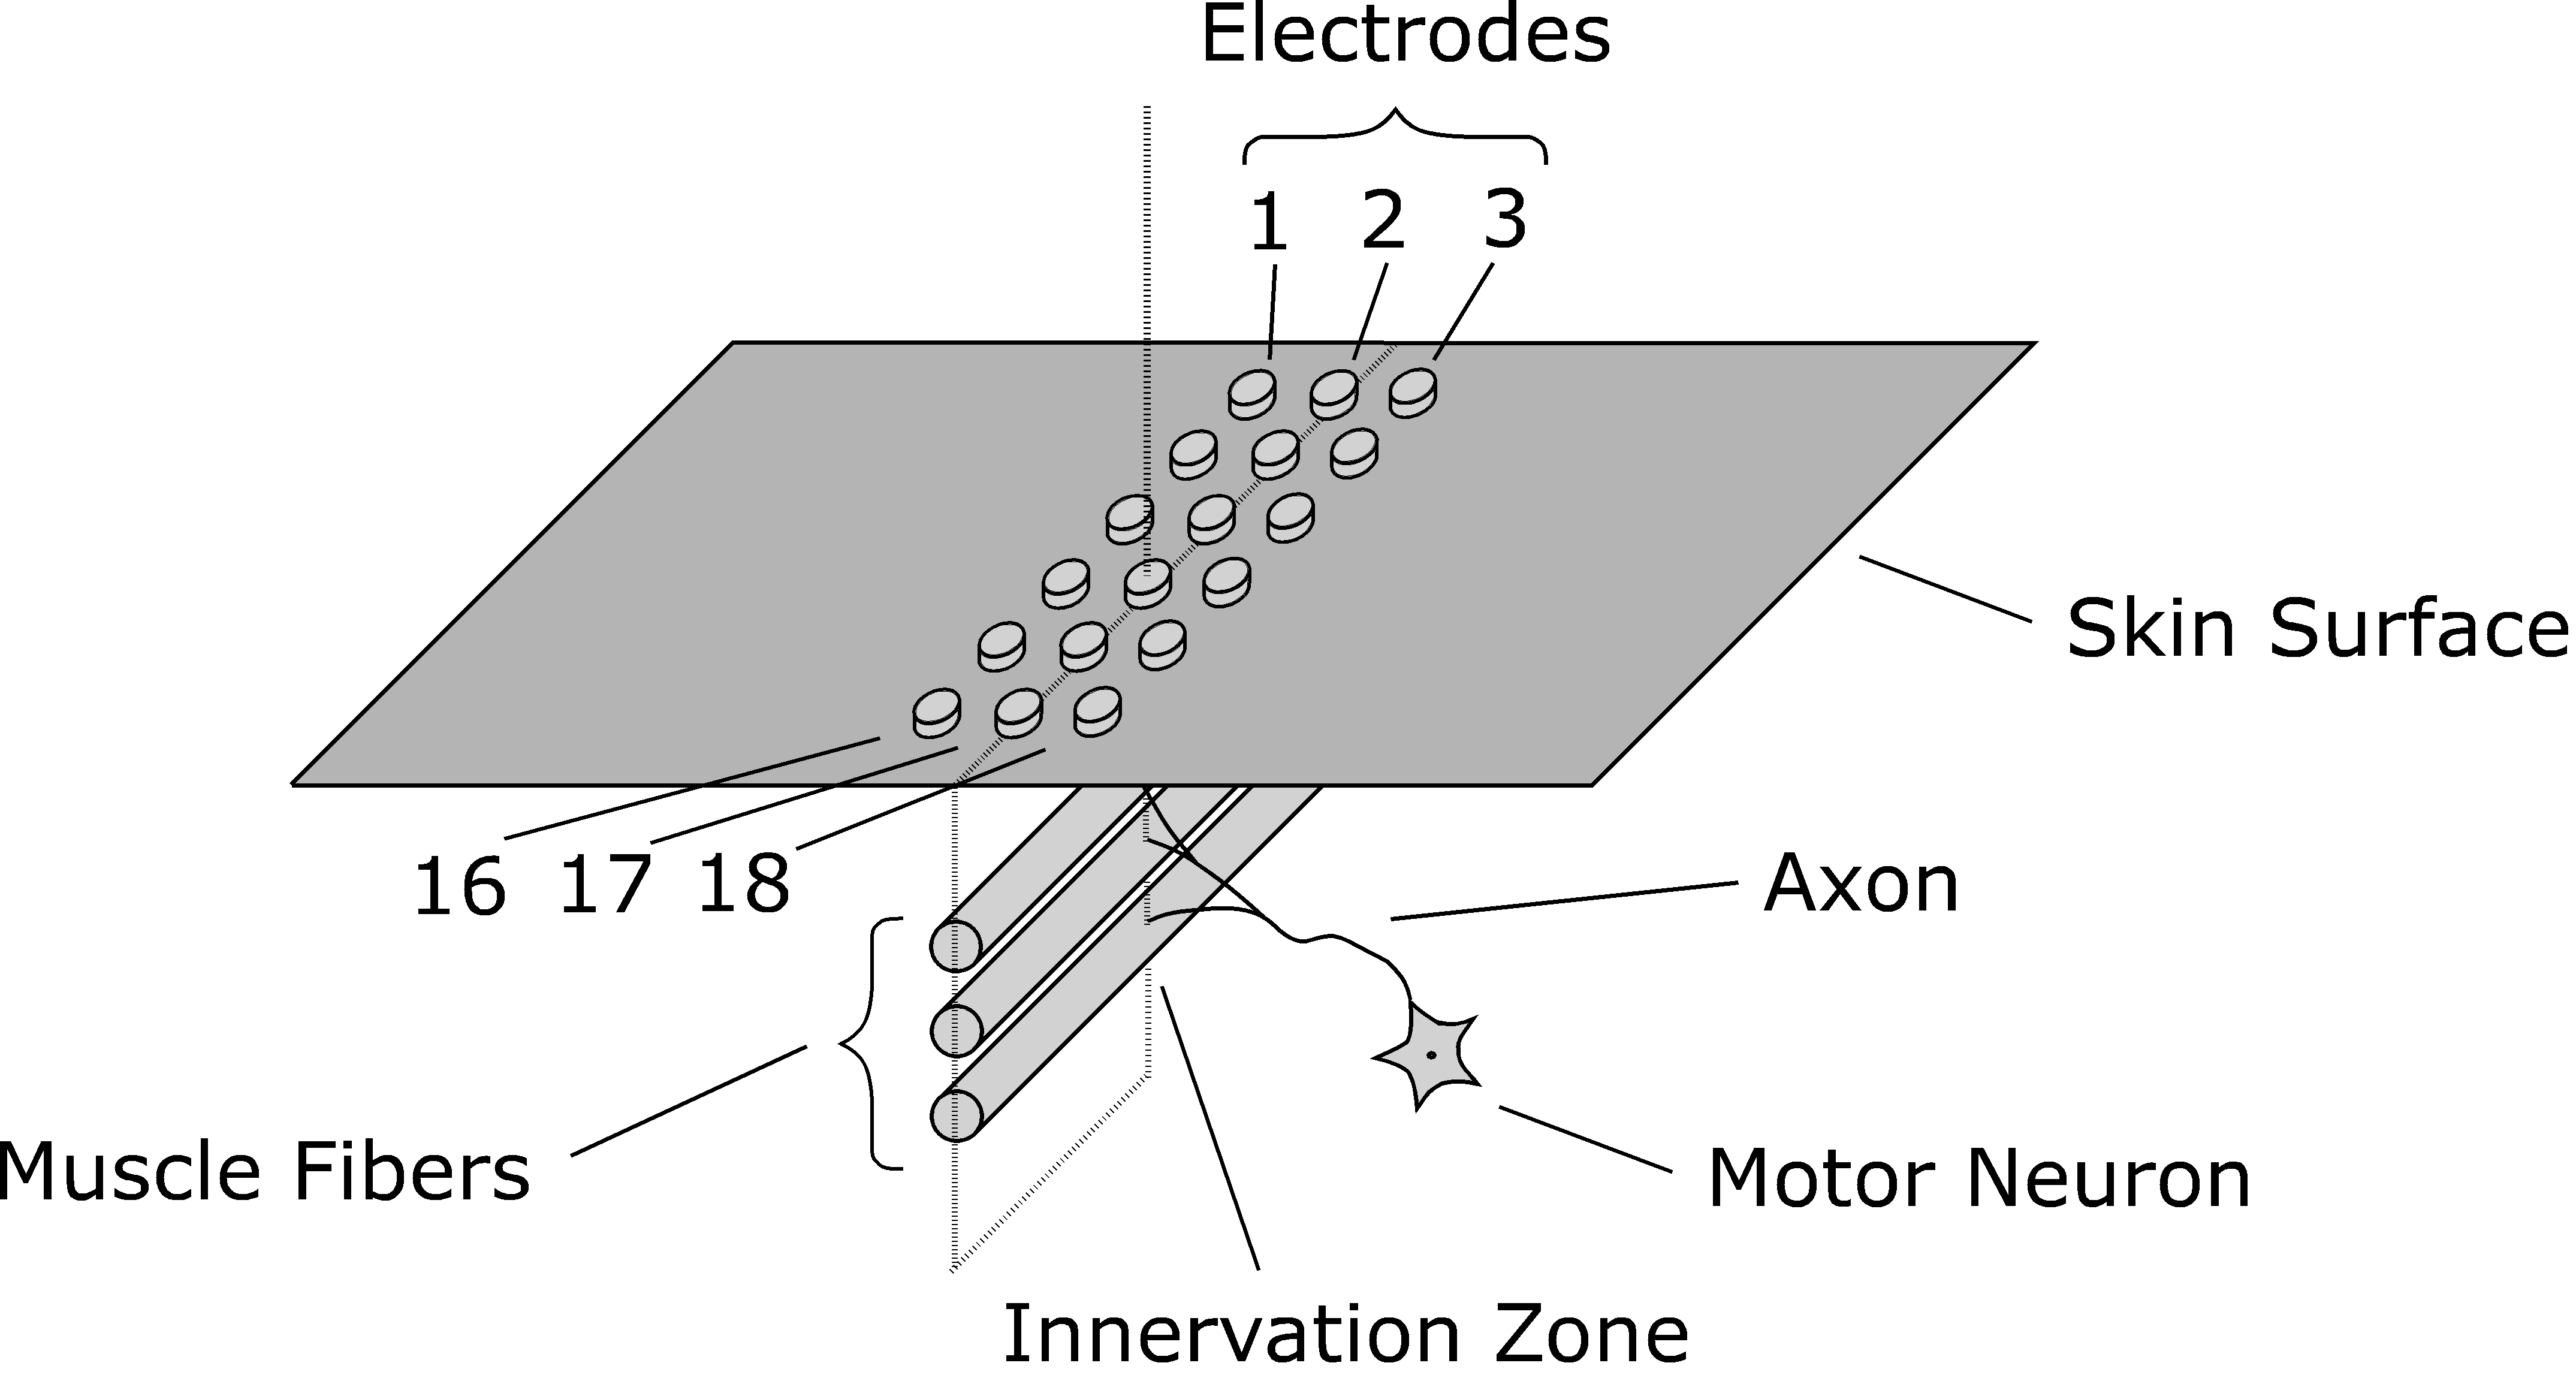
\includegraphics[width=12cm]{sfap-schematic}
  \caption[Geometry of Single Fiber Action Potential (SFAP) measurements]{Schematic of the geometry in \acrfull{sfap} measurements of human muscle fibers. Shown are three muscle fibers at different depths in the muscle tissue, and a regular grid of $18$ recording electrodes on the skin surface.}
  \label{fig:sfap-schematic}
\end{figure}

As opposed to \cref{fig:sfap-schematic}, which is included here as an external graphics file, \cref{fig:simple-schematic} shows a simple electrical schematic that is created completely in Latex, using the \swname{circuitikz} package.
\begin{figure}
  \centering
  \begin{circuitikz} \draw
    (0,0) to [V=$U_0$] (0,3)
    to [R=$R_I$, i=$I_R$] (3,3)
    to [R=$R_L$] (3,0)
    to [C=$C_P$] (0,0)
    ;
  \end{circuitikz}
  \caption{A simple electrical circuit, drawn in Latex using the \swname{circuitikz} package.}
  \label{fig:simple-schematic}
\end{figure}
This package is based on the powerful \swname{tikz} package which allows for drawing any kind of figure directly in Latex.
This bears a number of advantages:
\begin{itemize}
\item The resulting figures are vector graphics, i.e., they are small (hence not resulting in a final thesis pdf size of several MBs) and generally look good.
\item Font style and size is consistent with the rest of the document. This is a major problem when importing figures from other software, e.g., \swname{Matlab}. (Also compare \cref{fig:sfap-schematic}.)
\item Each figure created this way is completely reproducible and configurable in every aspect.
\end{itemize}
Another package that is also based on the \swname{tikz} package is the \swname{pgfplots} package which enables the user to create plots either completely in Latex, or import data from an external program (e.g., \swname{matlab}) and generate a nice-looking plot from this data using \swname{tikz} (with the advantages mentioned above).
\Cref{fig:rosenfalck} shows an example of two plots generated using the \swname{pgfplots} package.
\begin{figure}
  \centering
  \newcommand*{\scalefactor}{0.8}
  \begin{subfigure}[t]{.5\textwidth}
    \centering
    \begin{tikzpicture}
        \newcommand*{\Aros}{96}
  \newcommand*{\Bros}{-90}
  \begin{axis}[
    small,
    width = \scalefactor\textwidth,
    axis lines = left,
    x unit = mm,
    y unit = mV,
    xlabel = $z$,
    ylabel = $V$,
    xtick={0,5,10},
    ymin = -99,
    ymax = 49,
    extra y ticks = {\Bros},
    extra y tick labels = {$B$},
    ]
    % Right part of the expression
    \addplot [
    domain=-2:15, 
    samples=1000, 
    color=blue,
    ]
    {x>0 ? \Aros*x^3*e^(-x)+\Bros : \Bros};

    \draw[dashed] (-2,\Bros) -- (15,\Bros);
  \end{axis}
    \end{tikzpicture}
    \caption{$V_m(z)$}
    \label{fig:rosenfalck-1}
  \end{subfigure}%
  \begin{subfigure}[t]{.5\textwidth}
    \centering
    \begin{tikzpicture}
      \newcommand*{\Aros}{96}
\newcommand*{\Bros}{-90}
\pgfplotsset{set layers}
\begin{axis}[
  small,
  width = \scalefactor\textwidth,
  axis y line = left,
  axis x line* = bottom,
  x unit = mm,
  y unit = mV/mm,
  xlabel = $z$,
  ylabel = $\psi$,
  xmin = -15,
  xmax = 2,
  ymin = -79,
  ymax = 39,
  xtick = {-10, -5, 0},
  ]

  \addplot [
  domain=-15:2, 
  samples=1000, 
  color=blue,
  ]
  {x>=0 ? 0 : -3*\Aros*x^2*e^x-\Aros*e^x*x^3}
  node[pos = 0.03,
       pin = 70 : {$\psi$}] {};

\end{axis}

\begin{axis}[
  small,
  width = \scalefactor\textwidth,
  axis y line = right,
  axis x line = none,
  x unit = mm,
  y unit = mV/mm^2,
  xlabel = $z$,
  ylabel = $\psi'$,
  xmin = -15,
  xmax = 2,
  ymin = -59,
  ymax = 119,
  ]

  \addplot [
  domain=-15:2, 
  samples=1000, 
  color=purple,
  ]
  {x<0 ? -(6*x+6*x^2+x^3)*\Aros*e^x : 0}
  node[pos = 0.02,
       pin = 70 : {$\psi'$}] {};
\end{axis}                      

    \end{tikzpicture}
    \caption{$\psi(z)=\dd{z} V_m(-z)$ and $\psi'(z)$}
    \label{fig:rosenfalck-2}
  \end{subfigure}%
  \caption[Plots of Rosenfalck's model function for the \acrlong{iap}]{Plots of the \acrfull{iap} model function proposed by \textcite{rosenfalck69}.}
  \label{fig:rosenfalck}
\end{figure}

\section{Referencing}
In this chapter in particular (materials and methods), you should provide a lot of references, e.g., to scientific articles~\cite{farina99}, books~\cite{plonsey07}, book chapters~\cite{rodriguez-falces12}, PhD theses~\cite{fevotte03}, or software projects~\cite{r-project} that you used during the creation of your thesis.
Sometimes, you should explicitly name authors, such as \textcite{farina99}, who wrote a seminal article on the mathematical modelling of \gls{emg} measurements.
A bibliography can be created automatically (see the appendix for an example).

Note how the \gls{emg} acronym is clickable and leads to the definition of this acronym in the glossary.
This is one of the many features of the \swname{glossaries} package.

\subsection{This is a subsection}
See the source code for how this is achieved.

\subsubsection{This is a subsubsection}
Note that the different appearance of chapters, sections, subsection and subsubsections can be customized if desired.

\section{Equations}
If you are going to write more than a few equations in your thesis, it is highly recommendable to use macros to define each variable that occurs.
This way, if you decide to rename the velocity from $v$ to $v_0$ (see the source code of this section for how to include mathematical symbols like $v$ in normal text) everywhere in your thesis later on during the process of writing, you will only have to change the definition of the macro used for this variable.
For example, in
\begin{equation}
  \label{eq:1}
  \vel = \frac{\diff \loc}{\diff t}
\end{equation}
and
\begin{align}
  \label{eq:2}
  \acc &= \frac{\diff \vel}{\diff t} \nonumber \\
  &= \frac{\force}{\mass},
\end{align}
each of the variables is defined using a macro.
Always keep in mind that formulas should be treated as a normal part of a sentence and thus can and have to contain punctuation marks!
\emph{Never} should any sentence start with a mathematical symbol.
Finally, here comes an example of how to reference equations \eqref{eq:1} to \eqref{eq:2}.

\section{Pseudo Code}
Algorithm \ref{alg:euclid} is an example of how pseudo code can be represented in Latex.
Of course there are, as with anything in Latex, many options available to achieve this goal.
Here, the \swname{algpseudocode} package is employed.
\begin{algorithm}
  % Example code due to
  % http://tex.stackexchange.com/a/230789/64293
    \caption{Euclid's algorithm}
    \label{alg:euclid}
    \begin{algorithmic}[1] % The number tells where the line numbering should start
        \Procedure{Euclid}{$a,b$} \Comment{The g.c.d. of a and b}
            \State $r\gets a \bmod b$
            \While{$r\not=0$} \Comment{We have the answer if r is 0}
                \State $a \gets b$
                \State $b \gets r$
                \State $r \gets a \bmod b$
            \EndWhile\label{euclidendwhile}
            \State \textbf{return} $b$\Comment{The gcd is b}
        \EndProcedure
    \end{algorithmic}
\end{algorithm}




%%%%% Emacs-related stuff
%%% Local Variables: 
%%% mode: latex
%%% TeX-master: "../../main"
%%% End: 
